\documentclass[30pt,french]{report}

% This is the main framework I use for my LateX documents.
% main.tex by Alexis GRACIAS

%%%%%%%%%%%%%
% LIBRARIES %
%%%%%%%%%%%%%

\usepackage{babel}
\usepackage{hyperref} % Add links to the table of content, files and website
\usepackage{graphicx} % Required for inserting images
\usepackage{tabto}
\usepackage[dvipsnames]{xcolor} % Text color package and more colors
\usepackage{tikz} % Graph package
\usepackage{pdfpages}
\usepackage{caption}
\usepackage{subcaption}
%\usepackage[demo]{graphicx}
\usepackage[utf8]{inputenc}
\usepackage{amsmath,amsfonts,mathtools,stmaryrd} % Math libraries

\usepackage{listings} % required for specific languages
\lstset{ % Set listing package options
    language=bash, % choose the language of the code
    basicstyle=\fontfamily{pcr}\selectfont\footnotesize\color{red},
    keywordstyle=\color{black}\bfseries, % style for keywords
    numbers=none, % where to put the line-numbers
    numberstyle=\tiny, % the size of the fonts that are used for the line-numbers     
    backgroundcolor=\color{white},
    showspaces=false, % show spaces adding particular underscores
    showstringspaces=false, % underline spaces within strings
    showtabs=false, % show tabs within strings adding particular underscores
    frame=single, % adds a frame around the code
    tabsize=2, % sets default tabsize to 2 spaces
    rulesepcolor=\color{gray},
    rulecolor=\color{black},
    captionpos=b, % sets the caption-position to bottom
    breaklines=true, % sets automatic line breaking
    breakatwhitespace=false, 
}

%\usepackage{eso-pic,lipsum}
%\AddToShipoutPicture{%
%	\AtTextCenter{%
%		\fboxsep5mm \fboxrule=0.8pt
%		\makebox(0,0)[c]{\fbox{\rule{0pt}\textheight\rule\textwidth{0pt}}}%
%	}%
%}

%%%%%%%%%%%%
% COMMANDS %
%%%%%%%%%%%%
\makeatletter 

\lstset{aboveskip=\baselineskip,belowskip=\baselineskip,basicstyle=\ttfamily} % Formating line break after bash commands

% Get rid of 0. chapter's number
\renewcommand{\thesection}{%
  \ifnum\c@chapter<1 \@arabic\c@section
  \else \thechapter.\@arabic\c@section
  \fi
}


% Rules for \bar{x} and \overline{x} commands
\newcommand*{\Xbar}{}%
\DeclareRobustCommand*{\Xbar}{%
  \mathpalette\@Xbar{}%
}

\newcommand*{\@Xbar}[2]{%
  % #1: math style
  % #2: unused (empty)
  \sbox0{$#1\mathrm{X}\m@th$}%
  \sbox2{$#1X\m@th$}%
  \rlap{%
    \hbox to\wd2{%
      \hfill
      $\overline{%
        \vrule width 0pt height\ht0 %
        \kern\wd0 %
      }$%
    }%
  }%
  \copy2 %
}

\makeatother

%%%%%%%%%%%%%%%%%%%%%%
% DOCUMENTS SETTINGS %
%%%%%%%%%%%%%%%%%%%%%%
% Fist page
\title{\Huge Fiche de révision Commande des Systèmes Dynamiques}
\author{\LARGE Alexis GRACIAS}
\date{\Large \today}

% Document
\begin{document}
\maketitle
\Large \tableofcontents

%%%%%%%%%%%
% INCLUDE %
%%%%%%%%%%%

\include{Oraganisation_du_cours}
\chapter{Notions d'estimation}
\section{Rappels des cours de 1A}
\subsection{Espace de Hilbert}
\begin{definition}{Espaces de Hilbert}{Espaces de Hilbert}
    Un espace de Hilbert est un \textbf{espace préhilbertien complet}, c'est à dire un \textbf{espace de Banach} dont la norme $||.||$ découle d'un \textbf{produit scalaire} ou \textbf{hermitien} par la formule suivante :
    \begin{equation}
        ||x|| = \sqrt{\langle x,x \rangle}
    \end{equation}
\end{definition}
\begin{definition}{Espaces de Banach}{Espaces de Banach}
    Un espace de Banach est un \textbf{espace vectoriel complet et normé} sur un sous corps $\mathbb{K}$ de $\mathbb{C}$ ($\mathbb{R}$ ou $\mathbb{C}$), peut importe la norme.
\end{definition}
\noindent \textbf{En d'autres termes, un espace de Hilbert est un espace vectoriel complet muni d'une norme définie par un produit scalaire.}
\subsection{Espace Lp}
\begin{definition}{Espaces $L^{p}[a,b]$}{Espaces Lp}
    Espace vectoriel des fonctions $p$ intégrables au sens de \textbf{Lebesgue} sur $[a,b]$. i.e.
    \begin{equation}
        \int_{a}^{b}{|f(t)|^{p}dt} 
    \end{equation}
    converge, avec la norme $L^{p}$: 
    \begin{equation}
        ||f||_{p} = \sqrt[\frac{1}{p}]{\int_{a}^{b}{|f(t)|^{p}dt}}
    \end{equation}
\end{definition}
\newpage
\subsection{Précisions}
\begin{definition}{Espace vectoriel normé}{Espace vectoriel normé}
    Un K-espace vectoriel $E$ est dit normé si il est muni d'une norme, c'est-à-dire d'une application $\mathcal{N} : E \rightarrow \mathbb{R}^{+}$ qui satisfait les conditions suivantes :
    \begin{itemize}
        \item \textbf{Séparation}
        \begin{equation}
            \forall x \in E, \mathcal{N}(x)=0 \implies x = 0_{E}  
        \end{equation} 
        \item \textbf{Homogénéité}
        \begin{equation}
            \forall (x,\lambda) \in E \times \mathbb{R}, \mathcal{N}(\lambda x) = |\lambda|\mathcal{N}(x)
        \end{equation} 
        \item \textbf{Sous-additivité (inégalité triangulaire)}
        \begin{equation}
            \forall (x,y) \in E^{2}, \mathcal{N}(x+y) < \mathcal{N}(x)\mathcal{N}(y)
        \end{equation} 
    \end{itemize}
\end{definition}
\begin{definition}{Espace métrique complet}{Espace métrique complet}
    Un espace métrique $(E,d)$ est dit complet si toute suite de Cauchy \footnote{
        Suite qui vérifie le critère de Cauchy, c'est-à-dire que les éléments de la suite se rapprochent uniformément entre-eux à l'infini, i.e. 
        \begin{equation}
            \forall \epsilon > 0, \exists (n_{0},p_{0}) \in \mathbb{N}^{2}, \forall n > n_{0}, \forall p > p_{0}, d(x_{n}, x_{p}) < \epsilon   
        \end{equation}
     } 
     converge dans ce même espace, c'est-à-dire :
    \begin{equation}
        \forall n \in \mathbb{N}, (x_{n})_{n \in \mathbb{N}} \in E, x_{n} \longrightarrow l \in E
    \end{equation}
\end{definition}
\begin{definition}{Espace métrique}{Espace métrique}
    On note $(E,d)$ un espace métrique ($E$ ensemble et $d$ la distance définie pour tout éléments de $E$). C'est un espace vectoriel au sein duquel la notion de distance est bien définie pour tout éléments de $E$. L'application $d$ satisfait les conditions suivantes :
    \begin{itemize}
        \item \textbf{Symétrie}
        \begin{equation}
            \forall (x,y) \in E^{2}, d(x,y) = d(y,x)
        \end{equation} 
        \item \textbf{Séparation}
        \begin{equation}
            \forall (x,y) \in E^{2}, d(x,y) = 0 \Longleftrightarrow x = y
        \end{equation} 
        \item \textbf{Inégalité triangulaire}
        \begin{equation}
            \forall (x,y,z) \in E^{3}, d(x,y) < d(x,z) + d(z,y)
        \end{equation} 
    \end{itemize}
\end{definition}
\newpage
\subsection{Probabilités}
\begin{definition}{Espaces probabilisé}{Espaces probabilisé}
    Un espace probabilisé est constitué d'un \textbf{espace probabilisable} et d'une \textbf{mesure de probabilité}, noté $(\Omega, \mathcal{A}, \mathbb{P})$ avec : \newline
    \begin{itemize}
        \item $\Omega$ : l'univers, l'espace des observations ou espace des évènements élémentaires
        \item $\mathcal{A}$ est une \textbf{tribu} sur $\Omega$
        \item $\mathbb{P}$ : mesure de probabilité \newline
    \end{itemize}
    \noindent tel que $\mathbb{P}(\Omega)=1$ et $\forall A \in \mathcal{A}$, $\mathbb{P}(A)$ est appelé \textit{probabilité de l'évènement $A$}
\end{definition}
\begin{definition}{Espaces probabilisables}{Espaces probabilisables}
    Un espace probabilisable est noté $(\Omega, \mathcal{A})$, il est constitué de \textbf{l'univers} et de la \textbf{tribu} de cet univers.
\end{definition}
\begin{definition}{Mesure de probabilité}{Mesure de probabilité}
   La mesure de probabilité est définie par l'application $\mathbb{P} : \Omega \longrightarrow [0;1]$ telle que :
   \begin{itemize}
    \item $\mathbb{P}(\Omega) = 1$ 
    \item $\mathbb{P}(\{\}) = 0$
    \item \textbf{$\sigma$-additivité} : $\forall $ collection dénombrable $\{ A_{i} \}$ d'ensemble disjoints :
    \begin{equation}
        \mathbb{P}(\bigcup_{I \in \mathcal{I}} A_i) = \sum_{I \in \mathcal{I}} \mathbb{P}(A_{i})
    \end{equation}
   \end{itemize}
\end{definition}
\subsection{Schématiquement}
\begin{center}
    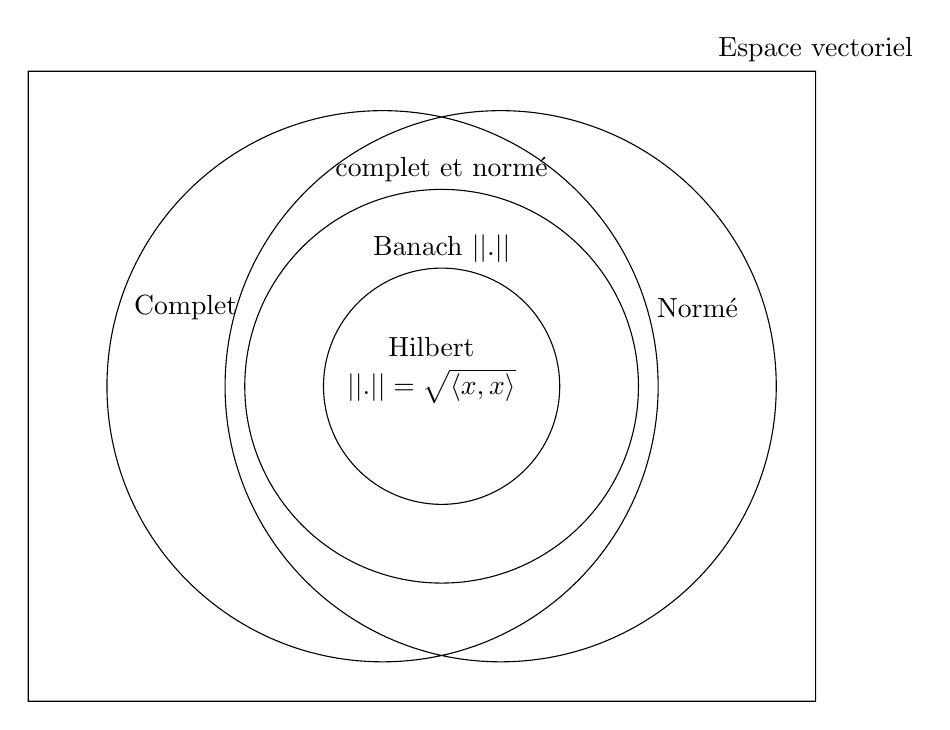
\begin{tikzpicture}[fill=red]
        \centering
        % outline
        \draw (-0.5,-1) circle (3.5) (0,1)  node at (-3,0) {Complet}
              (1,-1) circle (3.5) (1,1)  node  at (3.5,0) {Normé}
              (1,-1) circle (0) (1,0)  node  at (0.25,1.75) {complet et normé}
              (0.25,-1) circle (2.5) (1,1)  node at (0.25,0.75) {Banach $||.||$}
              (0.25,-1) circle (1.5) (1,0)  node at (0.12,-0.5) {Hilbert}
              (0.25,-1) circle (0) (1,0)  node at (0.12,-1)  {$||.|| = \sqrt{\langle x,x \rangle}$}
              (-5,-5) rectangle (5,3) node [text=black,above] {Espace vectoriel};
    \end{tikzpicture}
\end{center}
\newpage
\section{Transformée de Fourrier continue}

\section{Transformée de Fourrier discrète}

\newpage
\section{Estimation}
\subsection{Notions et définitions de base}
\noindent On cherche à reconstituer un signal aléatoire $\underline{x}$ ou $\underline{\theta}$ à partir de son observation, le vecteur $\underline{y}$. Par conséquent, les éléments $y_{i}$ du vecteur d'observation $\underline{y}$ sont des \textbf{VA} sur un espace probabilisé. On cherche alors une fonction $\widehat{\theta}$ tel que $x \circ y = \widehat{x}(\underline{y})$ soit la meilleure estimation de $\underline{x}$.
\begin{figure}[hbt!]
    \centering
    \includegraphics[scale=0.425]{Pics/Shanon.png}
    \caption{Modèle de transmission de Shanon}
\end{figure}

\noindent Mathématiquement, on a : 
\[ \underline{x} = 
\begin{bmatrix}
    x{0} & x_{1} & ... & x_{n} 
\end{bmatrix}
\in G
\]
\[ \underline{y} = 
\begin{bmatrix}
    y_{0} & y_{1} & ... & y_{n} 
\end{bmatrix}
\in F
\]
Avec :
\begin{itemize}
    \item $\underline{x}$ : \textbf{paramètre décisionnel} (aussi noté $\underline{\theta}$) : c'est le paramètre sur lequel est pris la décision. Il est peut être déterministe ou aléatoire. \newline
    \item $\underline{y}$ : \textbf{vecteur d'observation}. $(\Omega, \epsilon, P)$ est un espace probabilisé qui modélise l'expérience aléatoire permettant d'observer les signaux aléatoires rencontrés (i.e. $\underline{x}$). Par conséquent, $\underline{y} : \Omega \longrightarrow F$, soit $\underline{y} \in \mathcal{M}(\Omega, F)$ \footnote{i. e. $\underline{y}$ est une \textbf{VA} $\Longleftrightarrow \underline{y}$ est une fonction qui à tout évènement $\omega \in \Omega$ associe une valeur $y_{i} \in F$} \newline
    \item $(x_{i})_{i \in \mathbb{N}}$ et $(y_{i})_{i \in \mathbb{N}}$ : \textbf{variables aléatoires} de $\underline{x}$ et de $\underline{y}$ \newline
    \item $(G,\mathcal{G})$ et $(F,\mathcal{F})$ sont des espaces probabilisables. $F$ est \textbf{l'espace des observations} et $G$ \textbf{l'esapce des paramètres} \newline
\end{itemize}
\subsection{Estimateur}
\noindent Pour un \textbf{estimateur $\widehat{\theta}$}, le meilleur estimateur (ou filtre) de $\theta$ est donc l'application $\widehat{\theta}$:
\begin{equation}
    \large
    \tcbhighmath[fuzzy halo=0.5mm with electricultramarine!35!electricultramarine,arc=2pt,
    boxrule=0pt,frame hidden]{ 
        \widehat{\theta} : F \longrightarrow G, \\ \widehat{\theta} \circ y = \widehat{\theta}(\underline{y}) \in \mathcal{M}(F,G)
     } \nonumber
    \normalsize
\end{equation}
Avec $\mathcal{M}(F,G)$ l'ensemble des applications \textbf{mesurables} de $F$ dans $G$. \newline
\newpage
\subsection{Densité de probabilité conditionnelle - vraisemblance}
\noindent $(\Omega, \epsilon, P)$ est un espace probabilisé qui modélise l'expérience aléatoire (signaux aléatoires rencontrés) \newline
\noindent $\underline{y}$ est le vecteur d'observation qui admet une \textbf{densité} par rapport à $F$, de \textbf{mesure canonique}\footnote{Mesure canonique que l'on prend comme mesure de Lebesgue. \newline On a, pour $\underline{y} \in \mathcal{M}(\Omega, F)$ de mesure $d\underline{v} = d\mu(\underline{v})$, que $\forall y_{i} \in F, \mu(y_{i}) = P(\underline{y}^{-1}(y_{i}))$. De même, on note $d\underline{u} = dv(\underline{u})$ pour la mesure de l'espace décisionnel $\mathcal{G}$}, tandis que $\widehat{\theta}(\underline{y})$ est une VA à valeurs dans $G$, alors la \textbf{densité de probabilité conditionnelle de $\underline{y}$ sachant $\theta$ } s'exprime sous la forme :
\begin{equation}
    \large
    \tcbhighmath[fuzzy halo=0.5mm with electricultramarine!35!electricultramarine,arc=2pt,
    boxrule=0pt,frame hidden]{ 
        f_{\underline{y}|\theta}(\underline{v}|\theta), \forall \underline{v} \in F
     } \nonumber
    \normalsize
\end{equation}
On supposera dans le cours que la vraisemblance est connue (i.e. la loi de la VA est connue)
\subsection{Fonction de perte ou de coût}
C'est une application $L$ telle que :
\begin{equation}
    \large
    \tcbhighmath[fuzzy halo=0.5mm with electricultramarine!35!electricultramarine,arc=2pt,
    boxrule=0pt,frame hidden]{ 
        L : G \times G \longrightarrow \mathbb{R}, (\theta_{1},\theta_{2}) \mapsto L[\theta_{1},\theta_{2}] \nonumber
     } \nonumber
    \normalsize
\end{equation}
Pour un estimateur $\widehat{\theta}$ et $\underline{v} \in F$ donnés, $L[\widehat{\theta}(\underline{v}), \theta]$ représente le \textbf{coût de la décision} $\widehat{\theta}(\underline{v})$ quand la vraie valeur du paramètre décisionnel est $\theta$. Ce coût est généralement arbitraire. \newline
\subsection{Fonction de risque}
\noindent Fonction déterministe qui dépend de $\widehat{\theta}$ et $\theta$. C'est l'espérance de la perte entre la valeur du paramètre $\theta$ estimée et sa vraie valeur, sachant que $\theta$ vaut tant.
\begin{equation}
    \large
    \tcbhighmath[fuzzy halo=0.5mm with electricultramarine!35!electricultramarine,arc=2pt,
    boxrule=0pt,frame hidden]{ 
        \mathcal{R}(\widehat{\theta},\theta) = E[L(\widehat{\theta}(\underline{y}),\theta)|\theta] = \int_{F}{L[\widehat{\theta}(\underline{v}), \theta]f_{\underline{y}|\theta}(\underline{v}|\theta)}{d\underline{v}} \nonumber
     } \nonumber
    \normalsize
\end{equation}
Ici, l'objectif est de trouver une fonction $\widehat{\theta}$ qui minimise le risque, c'est-à-dire une fonction $\widehat{\theta}$ qui se rapproche le plus possible de sa vraie valeur.
\section{Point de vu Bayésien et non Bayésien}
\begin{itemize}
    \item \textbf{Non Bayésien} : $\theta$ est supposé déterministe, c'est à dire qu'il obéit à des lois non probabilistes \newline
    \item \textbf{Bayésien} : $\theta$ est supposé aléatoire et de loi connue \newpage
    \item \textbf{Paramétrique} : $\theta$ est aléatoire et de loi connue (i.e. Bayésien sans supposition) \newline
    \item \textbf{Non Paramétrique} : $\theta$ est aléatoire et de loi inconnue. \newline
\end{itemize}
\noindent Le point de vu \textbf{fréquentiste}, i.e. non paramétrique ne sera étudié dans le cadre de ce cours. Le point de vu Bayésien permet d'introduire d'autres notions telles que : \newline
\subsection{Risque moyen - $\theta$ Bayésien}
\noindent En adoptant le \textbf{point de vue Bayésien}, pour une \textbf{densité de probabilité a fortiori $f_{\theta}(u)$} du paramètre décisionnel, le risque moyen s'exprime sous la forme :
\begin{equation}
    \large
    \tcbhighmath[fuzzy halo=0.5mm with electricultramarine!35!electricultramarine,arc=2pt,
    boxrule=0pt,frame hidden]{ 
        \overline{R}(\widehat{\theta}) = E[R(\widehat{\theta}), \theta] = \int_{G}{R(\widehat{\theta},u)}f_{\theta}(u)du = \int_{F}{H_{c}(\underline{v})f_{y}(\underline{v})}d\underline{v}
     } \nonumber
    \normalsize
\end{equation}
Avec
\begin{equation}
    \large
    \tcbhighmath[fuzzy halo=0.5mm with electricultramarine!35!electricultramarine,arc=2pt,
    boxrule=0pt,frame hidden]{ 
        H_{c}(\underline{v}) =  \int_{G}{L[\widehat{\theta}(\underline{v}), u]f_{\theta | y}(u|\underline{v})}du = E\{L[\widehat{\theta}(\underline{y}),\theta]|\underline{y}=\underline{v}\}
    } \nonumber
    \normalsize
\end{equation}
La ddp conditionnelle $f_{\theta | y}(u|\underline{v})$ devient la \textbf{densité de probabilité a posteriori} et la loi de $\underline{y}$ est \textbf{l'evidence}.
Le but est ici de trouver le $\underline{v} \in F$ qui minimise $H(\underline{v})$ \newline

\noindent \textbf{Exemple - coût quadratique} \newline
\noindent Supposons $G = \mathbb{R}, L[\widehat{\theta}, \theta] = (\widehat{\theta} - \theta)^{2}$. Pour $\underline{v} \in F$, calculer le risque conditionnel :
\begin{align}
    H(\underline{v}) &= E[(\widehat{\theta} - \theta)^{2}|\underline{y} = \underline{v}] \nonumber \\
                     &= \widehat{\theta}^{2}(\underline{v}) - 2\widehat{\theta}(\underline{v})E[\theta | \underline{y} = \underline{v}] + E[\theta^{2} | \underline{y} = \underline{v}] \nonumber \\
                     &= (\widehat{\theta}(\underline{v}) - E[\theta | \underline{y} = \underline{v}])^{2} + E[(\theta - E[\theta | \underline{y}])^{2} | \underline{y} = \underline{v}] \nonumber
\end{align}
On obtient une équation quadraitque en $\widehat{\theta}(\underline{y})$ à résoudre. Le minimum de $H$ est atteint en 
\begin{equation}
    \widehat{\theta}(\underline{v}) = E[\theta | \underline{y} = \underline{v}] = \int_{G}{u f_{\theta | \underline{y}}(u | \underline{v}du)} \nonumber
\end{equation}
\subsection{Risque moyen - $\theta$ non Bayésien}
D'un \textbf{point de vue non Bayésien}, on utilise plutôt le maximum de vraisemblance : 
\Large
\begin{equation}
    \widehat{\theta}(\underline{y}) = arg (max f_{\underline{y} | \theta}(\underline{v}| \theta)) \nonumber
\end{equation}
\normalsize
En effet, pour $\theta$ déterministe, on définit :
\begin{itemize}
    \item \textbf{Le biais} : $B(\widehat{\theta}) = E[\widehat{\theta}] - \widehat{\theta}$
    \item \textbf{La variance} : $V(\widehat{\theta}) = E[\widehat{\theta}^{2}] - E[\widehat{\theta}]^{2}$
\end{itemize}
\newpage
\section{Estimation en moyenne quadratique (EMQ)}

\newpage
\section{Estimation linéaire en moyenne quadratique (ELMQ)}
\noindent D'un point de vue Bayésien, on prend un coût quadratique et on suppose $\underline{x}, \underline{y} \in L^{2}(P) \times L^{2}(P)^{n}$ avec :
\[
\underline{y} = 
\begin{bmatrix}
    y_{1} & ... & y_{n}    
\end{bmatrix}
^{H}\] \footnote{$H$ est ici l'opérateur transpose définit sur $H_{L}$, le sous-espace des observations filtrées avec contrainte, qui sera définit juste après.}. Le problème est de trouver l'estimateur $a^{H} : \mathbb{C}^{n} \longrightarrow \mathbb{C}$ tel que : 
\begin{equation}
    \widehat{x}_{L} = a^{H}\underline{y} \nonumber
\end{equation} 
soit la meilleure estimation de $\underline{x}$ et $a^{H}$ désigne la transposée de la matrice $a$ dans le \textbf{sous-espace des observations filtrées avec contraintes linéaires} $H_{L}[\underline{y}]$ tel que : 
\begin{equation}
    \large
    \tcbhighmath[fuzzy halo=0.5mm with electricultramarine!35!electricultramarine,arc=2pt,
    boxrule=0pt,frame hidden]{ 
        H_{L}[\underline{y}] := \{z \in L^{2}(P), \exists \underline{\omega} \in \mathbb{C}^{n}, z = \underline{\omega}^{H}\underline{y}\}
    } \nonumber
    \normalsize
\end{equation}
$\widehat{x_{L}} \in H_{L}[\underline{y}]$ est l'élément qui minimise la distance à $\underline{x}$.

\newpage
\section{Estimation affine en moyenne quadratique}

\section{Estimations en moyenne quadratique avec contraintes linéaires}

\section{Estimation non-Bayésienne}
\chapter{Marchés et régulations}
\section{La concurrence en Europe}
La politque globale de l'Europe est de mettre en place la concurrence partout ou cela est possible. En effet, la mise en concurrence des entreprises permet de faire baisser les prix pour les consommateurs et donc de réduire l'inflation. Cependant, la concurrence parfaite n'existe pas. Il faut donc que l'Europe puisse appliquer plusieurs politiques pour \textbf{réguler} ces phénomènes. Il y a une surveillance des insitutions visant à réduire les "monopoles naturels", à instaurer des politiques environnementales... \newpage

\subsection{Loi de l'offre et la demande}
\begin{center}
    \includegraphics[scale=0.7]{Pics/Offre_et_demande.png}    
\end{center}
$(Offre \searrow + demande = cste) \implies Prix \nearrow$ \newline
$(Offre \nearrow + demande = cste) \implies Prix \searrow$ \newline
$(Demande \searrow + offre = cste) \implies Prix \searrow$ \newline
$(Demande \nearrow + offre = cste) \implies Prix \nearrow$
\subsection{Courbe de l'offre en situation de concurrence}
\begin{center}
    \includegraphics[scale=0.8]{Pics/Courbe_de_l_offre.png}
\end{center}
\newpage
\subsection{Elasticité-prix $\epsilon$ de la demande}
\begin{center}
    \fbox{\huge{$\epsilon = \frac{\frac{dQ}{Q}}{\frac{dp}{p}} = \frac{dQ}{dp}\frac{p}{Q}$}}   
\end{center}
Mesure de la variation de la quantité d'un produit par rapport à la variation de son prix
p : prix du produit \newline
q : quantité du produit
\begin{itemize}
    \item $\epsilon = 0 $ : inélasticité
    \item $\epsilon \in [-1;0[$ : faiblement élastique
    \item $\epsilon \in ]-\infty;-1]$ : élastique
\end{itemize}
\subsection{Elasticité à court et à long terme}
Il faut un certain  temps avant que la quantité d'un produit se stabilise face à une variation de prix
\begin{center}
    \includegraphics[scale = 1]{Pics/elasticite_court_et_long_terme.png}
\end{center}
\newpage
\subsection{Elasticité des prix croisés de la demande}
C'est la mesure de la déportation d'un produit A vers un produit B lorsque le prix de A augmente.
\begin{center}
    \huge{\fbox{$\epsilon_{i,j} = \frac{\frac{\partial Q_{i}}{Q_{i}}}{\frac{\partial p_{j}}{p_{j}}}=\frac{\partial Q_{i}}{\partial p_{j}}\frac{p_{j}}{Q_{j}}$}}
\end{center}
\begin{itemize}
    \item Si $\epsilon_{i,j} > 0 $: les biens sont substituables
    \item si $\epsilon_{i,j} < 0 $: les biens sont complémentaires
\end{itemize}
\begin{center}
    \includegraphics[scale=0.8]{Pics/elasticite_prix_croises.png}
\end{center}
\subsection{Elasticité revenu de la demande}
C'est la mesure de l'évolution du revenu réel du consommateur et de l'évolution de la quantité de produit.
\begin{center}
    \huge{\fbox{$\epsilon_{R} = \frac{\frac{dQ}{Q}}{\frac{dp}{p}}=\frac{dQ}{dp}\frac{p}{Q}$}}
\end{center}
\begin{itemize}
    \item Si $\epsilon_{R} > 1 $: le bien est dit \textbf{de luxe}
    \item si $\epsilon_{R} < 0 $: les biens est dit \textbf{inférieur}
\end{itemize}
\newpage
\section{La technologie de l'entreprise}
Conditions de production de l'entreprise :
\begin{itemize}
\item facteurs de production : 
    \begin{itemize}
        \item $K$ : capital\footnote{Ex : nombre d'heures de fonctionnenment des machines}
        \item $L$ : travail \footnote{Ex : nombre d'heures de travail}
        \item w : taux de salaire horraire
        \item r : coût horraire du capital
    \end{itemize}
\item Fonction de production
    \begin{itemize}
        \item $Q = f(K,L)$
    \end{itemize}
\item Fonction coût de l'entreprise
    \begin{itemize}
        \item $CF$ : coût fixe
        \item $CV(Q)$ : coût variable
    \end{itemize}
\end{itemize}
Fonction de coût total :
\begin{center}
    \Large{\fbox{$CT(Q) = CF + CV(Q)$}}
\end{center}
Fonction de coût moyen :
\begin{center}
    \Large{\fbox{$CM(Q) = \frac{CT(Q)}{Q} = \frac{CF}{Q} + \frac{CV(Q)}{Q}$}}
\end{center}
Fonction de coût marginal :
\begin{center}
    \Large{\fbox{$Cm(Q) = \frac{dCT(Q)}{dQ} = \frac{dCV(Q)}{dQ}$}}
\end{center}
\newpage
\section{Concurrence parfaite}
Comportement de la firme en situation de concurrence :
\begin{itemize}
    \item $\pi$ : profit de l'entreprise
\end{itemize}
Maximisation du profit de l'entreprise, en situation de \textbf{price taker}\footnote{L'entreprise est "preneuse de prix" : elle n'a pas le pouvoir d'influencer les prix sur le marché} : 
\begin{center}
    \Large{\fbox{$\max \pi (Q) = pQ - CT(Q)$}}
\end{center}
Condition de premier ordre :
\begin{center}
    \Large{\fbox{$\frac{d\pi(Q)}{dQ} = 0$}}
\end{center}
\begin{center}
    \Large{$\frac{d\pi(Q)}{dQ} = p - \frac{dCT(Q)}{dQ} = 0 \Longleftrightarrow p - C_{m}(Q) = 0$}
\end{center}
L'entreprise produit une quantité $Q$ tq : \Large{$p=C_{m}(Q)$} \newline

Comportement des entreprises sur un marché : plus il y a des opportunités dans un secteurs, plus les entreprises vont vouloir entrer dans ce secteur, ce qui a pour conséquences d'augmenter l'offre et donc de faire baisser les prix. \newline
Conditions de la concurrence parfaite:
\begin{center}
    \begin{itemize}
    \item Atomicité
    \item Biens homogènes
    \item libre entrée
    \item information parfaite
    \item Biens exclusifs
\end{itemize}
\end{center}
\newpage
\subsection{Dynamique de la concurrence parfaite}
Au bout d'un temps suffisament long, les profits $\pi$ des entreprises sont nuls et $p=CM=C_{m}$
\begin{center}
    \includegraphics[scale=0.8]{Pics/dyn_concu_parfaite.png}
\end{center}
Rendements de la fonction de production : \newline
La fonction de production a 
\begin{itemize}
    \item Un rendement constant si :
    \begin{center}
        \Large{\fbox{$\lambda Q = f(\lambda K, \lambda L)$ avec $\lambda>1$}}
    \end{center}
    \item Un rendement décroissant si :
    \begin{center}
        \Large{\fbox{$\lambda Q < f(\lambda K, \lambda L)$}}
    \end{center}
        \item Un rendement croissant si :
    \begin{center}
        \Large{\fbox{$\lambda Q > f(\lambda K, \lambda L)$}}
    \end{center}
\end{itemize}
Fonction à rendement constant (fonction de Cobb-Douglas)
\begin{center}
    \Large{$Q = K^{\alpha}L^{\alpha}$}
\end{center}
\newpage
\subsection{Surplus du consommateur}
le surplus du consommateur est la mesure du taux de satisfaction client. C'est la différence entre le prix qu'il aurai payé pour le produit et le prix qu'il paye réellement.

avec :
\begin{itemize}
    \item $S$ : satisfaction
    \item $Q^{*}$ : quantité échangée
    \item $p^{*}$ : prix échangé
\end{itemize}
\begin{center}
    \includegraphics[scale=0.8]{Pics/surplus_consommateur.png}
\end{center}
\newpage
\section{Les défaillances du marché}
\subsection{Biens économiques}
Biens économiques : ils sont rivaux ou non, avedc un certain degré d'exclusivité
\begin{itemize}
    \item \textbf{Bien rival} : deux agents ne peuvent pas en bénéficier en même temps de ce bien \footnote{Bien rival = bien exclusif - ex : une voiture, tragédie des biens communs $\neq$ biens non-rivaux}
    \item \textbf{Bien exclusif} : bien que peut disposer l'agent que s'il paye le prix \footnote{ex : chaîne de télévision, logiciel, biens publics $\neq$ biens non-exclusifs}
\end{itemize}
Les biens et services de consommation privée traditionnelle sont les deux à la fois.
\subsection{Externalité}
C'est un effet subit par un agent économique au cours d'une action de consommation ou de production \footnote{Ces externalités sont trop ou pas assez produites, en fonciton de leurs types : il faut alors taxer et/ou subventionner certaines externalités pour les réguler.}
\begin{itemize}
    \item \textbf{Externalité positive} : effets de la R\&D, recherche publique sur la R\&d, recherche privée
    \item \textbf{Externalité négative} : effet de la pollution dûs aux rejets d'une usine
\end{itemize}
\begin{center}
    \includegraphics[scale=0.7]{Pics/defaillance_marche.png}
\end{center}
\newpage
\section{Le monopole}
\subsection{Comportement de l'entreprise}
Comportement de l'entreprise en situation de monopole
\begin{itemize}
    \item $\pi$ : profit de l'entreprise
    \item $Q(p)$ : fonction de demande
\end{itemize}
Maximisation du profit de l'entreprise, en situation de \textbf{price maker}\footnote{C'est l'entreprise qui fixe les prix}
\begin{center}
    \Large{\fbox{$max \pi(Q) = p(Q)Q - CT(Q)$}}
\end{center}
Condition de premier ordre :
\begin{center}
    \Large{\fbox{$\frac{d\pi(Q)}{dQ}=0$}}
\end{center}
\begin{center}
    \Large{$\frac{d\pi(Q)}{dQ} = \textcolor{BrickRed}{\frac{dp(Q)}{dQ}Q + p(Q)} - \textcolor{green}{\frac{dCT(Q)}{dQ}} = 0$}
\end{center}
\begin{itemize}
    \item\fbox{\textcolor{BrickRed}{$\frac{dp(Q)}{dQ}Q + p(Q) = R_{m}(Q)$}} la recette marginale \newline
    \item \textcolor{green}{$\frac{dCT(Q)}{dQ}$} le coût marginal \newline
    \item $\epsilon = \frac{dQ}{dp}\frac{p}{Q}$ (pour rappel)
\end{itemize}
Donc
\begin{center}
    $R_{m}(Q) = \frac{dp(Q)}{dQ}Q + p(Q) = \frac{1}{\epsilon}p(Q) + p(Q)$
\end{center}
on a alors : 
\begin{center}
    \Large{\fbox{$p(Q)(1+\frac{1}{\epsilon}) = C_{m}(Q)$}}
\end{center}
\newpage
Prix de monopole :
\begin{center}
    \LARGE{\fbox{$p(Q) = \frac{C_{m}(Q)}{1+\frac{1}{\epsilon}}$}}
\end{center}
En considérant la demande élastique (marché sur une échelle de temps longue soit $\epsilon \in ]-\infty;-1]$) :
\begin{center}
    \Large{$p^{M} = \frac{C_{m}(Q)}{1+\frac{1}{\epsilon}} > C_{m}(Q) = p^{C}$}
\end{center}
\begin{itemize}
    \item $p^{M}$ : prix du marché en situation de monopole
    \item $p^{C}$ : prix du marché en situation de concurrence
\end{itemize}
Marge :
\begin{center}
    \Large{\fbox{$M = \frac{p^{M}}{C_{m}}$}}
\end{center}
Taux de marge :
\begin{center}
    \Large{\fbox{$T_{m} = \frac{p^{M} - C_{m}}{C_{m}}$}}
\end{center}
\subsection{L'inefficience du monopole}
\begin{center}
    \includegraphics[scale=0.7]{Pics/Inefficience_monopole.png}
\end{center}
\newpage
\section{Les interractions stratégiques (ententes)}
Les situations de concurrence et de monopole sont deux structures de marché extrêmes et ne reflètent pas la réalité. En efft, il existe des phénomènes d'interdépendance et de startégies d'entreprises qui mènent à des ententes entres entreprises. \newline

\textbf{\textcolor{BrickRed}{Oligopole}} : nombre limité de grandes entreprises réalisant une part très importante de la production du secteur.
\newline
\begin{itemize}
    \item \textbf{Duopole de Cournot} : la quantité produite est la variable explicative de ces phénomènes \newline
    \item \textbf{Duopole de Bertrand} privilégie le prix \newline
    \item \textbf{Duopole de Stackelberg} : rôle des entreprises asymétrique (leader/follower)
\end{itemize}
\newpage
\subsection{Duopole de Cournot}
Soient deux entreprises qui produisent une quantité $q_{1}$ et $q_{2}$ de produits. Les coûts totaux sont $c_{1}q_{1}$ et $c_{2}q_{2}$. \newline
\begin{itemize}
    \item Quantité totale produite : \newline
    \textcolor{White}{.}
        \begin{center}
            \Large{\fbox{$Q = q_{1} + q_{2}$}}
        \end{center}
    \textcolor{White}{.}
    \item Fonction de demande inverse : \newline
    \textcolor{White}{.}
    \begin{center}
        \Large{\fbox{$p(Q) = p(q_{1} + q_{2}) = A - (q_{1} + q_{2})$}}
    \end{center}
    \textcolor{White}{.}
    \item Maximisation du profit de l'entreprise 1 et 2 : \newline
    \textcolor{White}{.}
        \begin{center}
            \begin{itemize}
                \Large{\fbox{$max  \pi(q_{1},q_{2}) = p(q_{1},q_{2})q_{1} - c_{1}(q_{1})$}} \newline
                \Large{\fbox{$max  \pi(q_{1},q_{2}) = p(q_{1},q_{2})q_{2} - c_{2}(q_{2})$}}
            \end{itemize}
        \end{center}
    \textcolor{White}{.}
    \item Conditions de premier ordre : \newline
    \textcolor{White}{.}
    \begin{center}
            \begin{itemize}
                \Large{\fbox{$\frac{\partial \pi_{1}(q_{1},q_{2})}{\partial q_{1}} = 0$}}
                \Large{\fbox{$\frac{\partial \pi_{2}(q_{1},q_{2})}{\partial q_{2}} = 0$}}
            \end{itemize}
    \end{center}
    \textcolor{White}{.}
\end{itemize}
\includegraphics[scale=0.8]{Pics/Duopole_cournot.png}
\newpage
\subsection{Duopole de Bertrand}
La valeur stratégique de l'entreprise est le prix. La fonction de demande du marché $D$ s'exprime en fonction du prix $p$ fixé par les deux entreprises.
Lorsque les prix fixés sont différents, on note $\forall i \in \{1,2\}, D_{i}$ la fonction demande du marché pour l'entreprise $i$. La demande sera adressée à l'entreprise ayant le prix le plus faible.
\[
\left \{
\begin{array}{c}
    D_{1} = D(p_{1}), D(p_{2}) = 0 ;p_{1} < p_{2}\\
    D_{1} = D_{2} = \frac{D(p_{1})}{2} =  \frac{D(p_{2})}{2} ;p_{1} = p_{2}\\
    D_{2} = D(p_{2}), D(p_{1}) = 0 ;p_{2} < p_{1}
\end{array}
\right.
\]
\begin{itemize}
    \item Si $c_{1} = c_{2} = c$, la maximisation du profit $\pi_{i}$ pour les entreprises est : \newline
    \textcolor{White}{.}
    \begin{center}
        \Large{\fbox{$\pi_{i}(q_{i}) = (p_{i} - c)q_{i}$ avec $CT_{i}(q_{i}) = cq_{i}$}}
    \end{center}
    \textcolor{White}{.}
    \item Si $CT{i}(q_{i}) = c_{i}q_{i}$ et $CT{j}(q_{j}) = c_{j}q_{j}$ avec $c_{i} < c_{j}$, la maximisation du profit $\pi_{i}$ de l'entreprise i est : \newline
    \textcolor{White}{.}
    \begin{center}
        \Large{\fbox{$\pi_{i}(q_{i}) = D(c_{j})(c_{j} - c_{i})$}}
    \end{center}
    \textcolor{White}{.}
    \item Le coût moins élevé de l'entreprise 1 permet de s'accaparer la demande. La maximisation du profit pour les deux entreprises mènent à $p_{1} = p_{2} = c$. \textbf{L'équilibre de Bertrand mène au même résultats que la concurrence parfaite : profits nuls pour les entreprises à condition que les deux entreprises agissent de la même manière}
\end{itemize}
\newpage
\subsection{Duopole de Stackelberg}
Dans le cas d'un duopole de Stackelberg, une entreprise est en position dominante, \textbf{leader} et l'autre la suit, elle est \textbf{follower}. L'entreprise \textbf{leader} prend des décisions que l'autre entreprise ne peut contester et \textbf{anticipe ses réactions}. \newline
\begin{itemize}
    \item Maximisation du profit du \textbf{follower} (entreprise 2) : \newline
    \textcolor{White}{.}
    \begin{center}
        \Large{\fbox{$
        max \pi_{2}(q_{1},q_{2}) = p(q_{1},q_{2})q_{2} - c_{2}q_{2}
        $}}
    \end{center}    \textcolor{White}{.}
    \item Conditions de premier ordre : \newline
    \textcolor{White}{.}
    \begin{center}
        \Large{\fbox{$
        \frac{\partial \pi_{2}(q_{1},q_{2})}{\partial q_{2}} = 0
        $}}
    \end{center}
    \textcolor{White}{.}
    \item Fonction de réaction (identique à celle du duopole de Cournot) : \newline
    \textcolor{White}{.}
    \begin{center}
        \Large{\fbox{$
        q_{2} = R_{2}(q_{1}) = \frac{A - c_{2} - q_{1}}{2}
        $}}
    \end{center}
    \textcolor{White}{.}
    \item L'entreprise 1 connaît la façon de réagir de l'entreprise 2 : \newline
    \textcolor{White}{.}
    \begin{center}
        \Large{\fbox{$
        max \pi_{1}(q_{1},q_{2}) = p(q_{1},q_{2})q_{1} - c_{1}q_{1}
        $}}
    \end{center}
    Sachant que :
    \begin{center}
        \Large{\fbox{$
        q_{2} = R_{2}(q_{1}) = \frac{A - c_{2} - q_{1}}{2}
        $}}
    \end{center}
    \textcolor{White}{.}
    \item Conditions de premier ordre : \newline
    \textcolor{White}{.}
    \begin{center}
        \Large{\fbox{$
        \frac{\partial \pi_{1}(q_{1},q_{2})}{\partial q_{1}} = 0
        $}}
    \end{center}
\end{itemize}
\newpage
On a alors : 
\begin{center}
    \Large{\fbox{$
    q_{1} = \frac{A - 2c_{1} + c_{2}}{2}
    $}}
    \Large{\fbox{$
    q_{2} = \frac{A - 2c_{1} + c_{2}}{4}
    $}}
\end{center} 
Les quantités produites par l'entreprise 2 étant anticipées par l'entreprise 1, \textbf{l'entreprise leader peut produire plus qu'en situation de duopole de Cournot tandis que l'entreprise 2 produit moins, ce qui souligne l'avantage qu'à l'entreprise 1 sur l'entreprise 2.}
\newpage
\subsection{Entente collusive ou cartel}
Les entreprises peuvent envisager des ententes entre elles : elles forment un cartel qui se comporte comme un monopole avec plusieurs établissements et prix. \textbf{\Large{Le but est de maximiser la somme des profits des entreprises}}\newline
Ce type d'entente \textbf{n'est pas stable} : il y a généralement des non-respects de ces ententes.
\begin{center}
    \Large{\fbox{$max \pi = \pi_{1} + \pi_{2} = p(q_{1},q_{2})(q_{1} + q_{2}) - C_{1}(q_{1}) - C_{2}(q_{2})$}}
\end{center}
Conditions de premier ordre :
\begin{center}
   \fbox{\Large{$\forall i \in \{1,2\},$} \huge{$\frac{\partial \pi}{\partial q_{i}} = 0$}}
\end{center}
A l'équilibre : \Large{{$C_{m_{1}} = C_{m_{2}}$} \newline

Matrice des décisions :
\begin{center}
    \includegraphics[scale=0.9]{Pics/Matrice_des_decisions.png}
\end{center}

\chapter{Commande des systèmes par approche d'état}
\section{\large{Rôle du correcteur}}
\label{Section omega et xi}
\begin{itemize}
    \item \textbf{\large{Stabilité}} : $S_{p}(A)\footnote{Spectre de la matrice d'évolution du système}$
    \item \textbf{\large{Rapidité}} :
    \begin{center}
        \fbox{\Large{$
        D = e^{-\frac{\pi \xi}{\sqrt{1-\xi^{2}}}}
        $}}
    \end{center}
        \begin{center}
        \fbox{\Large{$
        t_{m} = \frac{\pi}{\omega_{0}\sqrt{1-\xi^{2}}}
        $}} \footnote{Avec : \Large{$
        \textcolor{BrickRed}{\omega_{0}t_{m} =  3}
        $}}
    \end{center}
    \item \textbf{\large{Précision}} : erreur statique $\epsilon_{0}$
\end{itemize}
\begin{center}
    \includegraphics[scale=0.65]{Pics/SLI_Troubleshoot.png}
\end{center}
\newpage
\section{Retour d'état}
\begin{center}
    \includegraphics[scale=0.7]{Pics/retour_etat.png}
\end{center}
\subsection{Cas continu}
\large{Soit le système représenté en boucle ouverte :}
\begin{center}
    \fbox{\LARGE{$
    \dot x(t) = Ax(t) + Bu(t)
    $}} \newline 
    
    Avec : $x \in \mathbb{R}^{n}, u(t) \in \mathbb{R}$
\end{center}
\large{En boucle fermée, la commande par retour d'état impose \newline
$ u(t) = -Kx(t) + e(t)$, $e \in \mathbb{R}$. Il vient :}
\begin{center}
    \fbox{\LARGE{$
    \dot x(t) = (A - BK)x(t) + Be(t)
    $}}
\end{center}
\subsection{Cas discret}
\large{Soit le système représenté en boucle ouverte :}
\begin{center}
    \fbox{\LARGE{$
    x[k+1] = Fx[k] + Gu[k]
    $}} \newline 
    
    Avec : $x \in \mathbb{R}^{n}, u[k] \in \mathbb{R}$
\end{center}
\large{En boucle fermée, la commande par retour d'état impose \newline
$ u[k] = -Kx[k] + e[k]$, $e \in \mathbb{R}$. Il vient :}
\begin{center}
    \fbox{\LARGE{$
    x[k+1] = (F - GK)x[k] + Be[k]
    $}}
\end{center}
\newpage
\section{Calcul du retour d'état par placement des pôles}
\large{C'est le cacul de $K$ en choisissant les valeurs propres de $F - GK$. D'après le \textcolor{BrickRed}{théorème de Wonham : il existe une matrice K tq pour tout choix de valeurs propres SSI le système est totalement commandable.} \newline
(i.e. $\exists K \in M_{n}(\mathbb{R})$, on peut choisir les $\lambda_{i} \in S_{p}(A - BK)$ SII $\forall \lambda \in S_{p}(A), Re(\lambda) 0$)}
\subsection{Cas continu}
\begin{center}
    \fbox{\Large{$
x(t) = e^{(A - BK)(t-t_{0})}x(t_{0})
= \sum_{i=1}^{n}{\alpha_{i}e^{\lambda_{i}(t-t_{0})}}
$}} \footnote{$\lambda_{i}$ vp de $A - BK$ ($\lambda_{i} \in S_{p}(A-BK)$)}
\end{center}
\subsection{Cas discret}
\begin{center}
    \fbox{\Large{$
x[k] = (F - GK)^{k-k_{0}}x[k_{0}]
= \sum_{i=1}^{n}{\alpha_{i}\lambda_{i}^{(k-k_{0})}}
$}} \footnote{$\lambda_{i}$ vp de $F - GK$ ($\lambda_{i} \in S_{p}(F-GK)$)}
\end{center}
\subsection{Principe}
On cherche à avoir 
\[K = 
\begin{bmatrix}
    k_{1} & k_{2} & ... & k_{n}
\end{bmatrix}
\in \mathbb{R}^{n}
\]
tel que $\forall i \in \{1,n\}$, les $k_{i}$ sont les pôles de la fonction de transfert du système et les critères de commandabilité sont respectés soit :
\begin{center}
    \item $\forall \lambda_{i} \in S_{p}(A - BK),Re(\lambda_{i}) < 0$ \newline
\end{center} 

\newpage
\subsection{Calcul de $K$}
On veut choisir les $\lambda_{i}$ tel que $|\lambda I - (A - BK)| = \prod_{i=1}^{n}(\lambda - \lambda_{i})$ \newline
\begin{itemize}
    \item \textcolor{BrickRed}{Formule d'Ackerman} (si $dim(u) = 1$) : \newline
    \begin{itemize}
        \item \Large{$
            (\lambda - \lambda_{1})(\lambda - \lambda_{2})(\lambda - \lambda_{3})...(\lambda - \lambda_{n}) = \lambda^{n} + \alpha_{1}\lambda^{n-1} + ... + \alpha_{n-1}\lambda + \alpha_{n}
            $} \newline
        \item \Large{$
        P(A) = A^{n} + \alpha_{1}A^{n-1} + ... + \alpha_{n-1}A + \alpha_{n}I_{n} 
        $} \newline
        \item Soit : \newline
        \Large{$
        K = [ 0  0  ...  0  1 ][B | AB | A^{2}B | ... | A^{n-1}B]P(A)
        $} \newline
    \end{itemize}
    \item \textcolor{BrickRed}{Calcul à partir des valeurs propres} ($dim(u) quelconque$) \newline
    \begin{itemize}
        \item Trouver les $(v_{i})_{i \in \llbracket 1 , n \rrbracket}$ et $(w_{i})_{i \in \llbracket 1 , n \rrbracket}$ tel que : \newline
        \Large{$
        \forall i \in \llbracket 1 , n \rrbracket , (A - \lambda_{i}I_{n})v_{i} - Bw_{i} = 0_{n}
        $} \newline
        \item Soit : 
    \[K = 
    \begin{bmatrix}
        v_{1} & ... & v_{n}
    \end{bmatrix}
    \begin{bmatrix}
        w_{1} & ... & w_{n}
    \end{bmatrix}
    ^{-1}\]
    \end{itemize}
\end{itemize}
\subsection{Critères à respecter pour le choix des $\lambda_{i}$}
\begin{itemize}
    \item $\forall \lambda_{i} \in S_{p}(A - BK),Re(\lambda_{i} 0)$ \newline
    \item Les pôles dominants sont tels que $\forall \lambda_{i} \in S_{p}(A - BK), \newline
    \lambda_{dominant} = max_{i \in \llbracket 1 , n \rrbracket}(Re(\lambda_{i}))$ \footnote{Pour un système stable} \newline
    \item Plus les $\lambda_{i}$ sont éloignés des vp de A, plus les amplitudes des gains de $K$ et donc des commandes $u(t)$ sont forte
\end{itemize}
\newpage
\subsection{Exemple pour la formule d'Ackerman}
On considère une fonction de transfert d'ordre 2 tel que : 
\begin{center}
    \Large{$
        H(p) = \frac{K}{(p - p_{1})(p - p_{2})}
    $}
\end{center}
Avec $p_{1}$ et $p_{2}$ les pôles de la fonctionde transfert. On veut :  
\[
K = 
\begin{bmatrix}
    p_{1} & p_{2}
\end{bmatrix}
\] tel que : 
\begin{center}
\fbox{\Large{$
    |\lambda I_{2} - (A - BK) | = (\lambda - p_{1})(\lambda - p_{2}) = \lambda^{2} + 2\xi \omega_{0}\lambda + \omega_{0}^{2} 
$}}
\end{center}
\textbf{1.} On procède par identification :
\[
    \left \{
    \begin{array}{c @{=} c}
        1 & 1 \\
        2\xi \omega_{0} & -p_{1} - p_{2}\\
        \omega_{0}^{2} & p_{1}p_{2} 
    \end{array}
    \right.
\]
\textbf{2.} Les $\xi$ et $\omega_{0}$ sont trouvés grâce aux équations suivantes : 
\begin{center}
    \fbox{\Large{$
    D = e^{-\frac{\pi \xi}{\sqrt{1-\xi^{2}}}}
    $}}
\end{center}
    \begin{center}
    \fbox{\Large{$
    t_{m} = \frac{\pi}{\omega_{0}\sqrt{1-\xi^{2}}}
    $}} \footnote{Avec : \Large{$
    \omega_{0}t_{m} =  3
    $}}
\end{center}
\textbf{3.} En résolvant le système d'équations, on trouve la valeur des pôles de $K$ \newline

Pour une FT d'ordre 3, on considère :
\[
K = 
\begin{bmatrix}
    p_{1} & p_{2} & p_{3}
\end{bmatrix}
\]
On a alors l'équation suivante :
\begin{center}
    \Large{$
    |\lambda I_{3} - (A - BK) | = (\lambda - p_{1})(\lambda - p_{2})(\lambda - p_{3}) = \lambda^{3} + 2\xi \omega_{0}\lambda^{2} + 2\alpha \omega_{0}^{2}\lambda + \omega_{0}^{3} 
    $}    
\end{center}
Comme la valeur $\alpha$ n'est pas atteignable, ce système est résolu à l'aide de fonctions Matlab telles que \texttt{place}. \textbf{Pour une résolution complète, voir suspension EM, cours CSD03}.
\newpage
\section{Calcul du gain statique}
On ajoute un gain $k_{c}$ en entrée de boucle :
\begin{center}
    \includegraphics[scale=0.5]{Pics/retour_etat_KC.png}
\end{center}
De manière à satisfaire le critère de précision ($\epsilon_{s} = 0$) du
système bouclé : 
\subsubsection{Cas continu}
\Large{
    \[
\left \{
\begin{array}{c @{=} c}
    \dot x(t) & (A - BK)x(t) + Bk_{c}y_{c}(t)\\
    y(t) & Cx(t)
\end{array}
\right.
\]
\large{
Avec : $dim(y) = dim(u) = 1$\newline
En régime permettant, on veut $y(t) = y_{c}(t) = y_{c}$ \newline
Soit :}
\begin{center}
    \fbox{\Large{$
    k_{c} = \frac{-1}{C(A-BK)^{-1}B}
    $}}
\end{center} 
\subsubsection{Cas discret}
\Large{
\[
\left \{
\begin{array}{c @{=} c}
    x[k+1] & (F - GK)x[k] + Gk_{c}y_{c}[k]\\
    y[k] & Cx[k]
\end{array}
\right.
\]
\large{
Avec : $dim(y) = dim(u) = 1$\newline
En régime permettant, on veut $y(t) = y_{c}(t) = y_{c}$ \newline
Soit :}
\begin{center}
    \fbox{\Large{$
    k_{c} = \frac{-1}{C(I_{n}-F + GK)^{-1}G}
    $}}
\end{center} 
\footnote{Attention : l'erreur statique est non nulle si la perturbation est constante}
\subsection{perturbation constante et mesurable}
\large{
Ici, on cherche à modéliser l'influence d'une perturbation sur un système bouclé avec un gain statique determiné, de façon à mettre en évidence la remarque émise sur la page précédente.
\begin{center}
    \includegraphics[scale=0.5]{Pics/Perturbations.png}
\end{center}
\large{Système en boucle fermée :}
}
\Large{
    \[
\left \{
\begin{array}{c @{=} c}
    \dot x(t) & Ax(t) + Bu(t) + B'd(t)\\
    y(t) & Cx(t)
\end{array}
\right.
\]
\large{Commande :} \newline
$u(t) = -Kx(t) + k_{c}y_{c}(t) + k_{d}d(t)$
\large{système en boucle ouverte :}
\Large{
    \[
\left \{
\begin{array}{c @{=} c}
    \dot x(t) & (A - BK)x(t) + Bk_{c}y_{c}(t) + (Bk_{d} + B')d(t)\\
    y(t) & Cx(t)
\end{array}
\right.
\]
\large{En régime permettant, on veut toujours $y(t) = y_{c}(t) = y_{c}$ \newline
Soit :}
\Large{
    \[
\left \{
\begin{array}{c @{=} c}
    k_{c} & -[C(A - BK)^{-1}B]^{-1}\\
    k_{d} & -[C(A - BK)^{-1}B]^{-1}[C(A - BK)^{-1}B']
\end{array}
\right.
    \]}
\newpage
\subsection{Exemple : suspension magnétique}
On considère le système suivant :
\begin{figure}[hbt!]
    \centering
    \begin{subfigure}{.5\textwidth}
      \centering
      \includegraphics[width=1\linewidth]{Pics/suspension_magnetique.png}
      \caption{Schéma associé au système}
      \label{fig:sub1}
    \end{subfigure}%
    \begin{subfigure}{.7\textwidth}
      \centering
      \includegraphics[width=.4\linewidth]{Pics/AN_suspension_magnetique.png}
      \caption{Application numérique}
      \label{fig:sub2}
    \end{subfigure}
    \caption{Sytème}
    \label{fig:test}
\end{figure}
\begin{center}
    \Large{$
    L\frac{dI(t)}{dt} + RI(t) = U(t)
    $} \footnote{Loi des mailles}
    \newline

    \Large{$
    m\frac{d^{2}z}{dt} = c\frac{I(t)}{(x_{0} - z(t)^{2}} - mg = F_{m} - mg
    $} \footnote{PFD}
\end{center}
\large{
\textbf{Point d'équilibre $\overline{z} = 0$}
}
\large{
    \[
\left \{
\begin{array}{c @{=} c}
    \overline{U} & R\overline{I} \\
    c\frac{\overline{I}}{x_{0}^{2}} - mg & 0
\end{array}
\right.
\]}
soit :
\large{
    \[
\left \{
\begin{array}{c @{=} c}
    \overline{I} & \frac{mgx_{0}^{2}}{c} = i_{0} \\
    \overline{U} & R\overline{I} = Ri_{0}
\end{array}
\right.
    \]}
En linéarisant sur le point d'équilibre, on a :
\large{
    \[
    \left \{
\begin{array}{c @{=} c}
    I(t) & \overline{I} + i_{1}(t) \\
    U(t) & \overline{U} + u_{0}(t)
\end{array}
\right.
    \]}
\newpage
Equations du système :
\begin{center}
    \Large{$
    L\frac{di_{1}(t)}{dt} + Ri_{1}(t) = u_{1}(t)
    $} 
    \newline

    \Large{$
    m\frac{d^{2}z}{dt} = g\frac{i_{1}(t)}{(i_{0}} + \frac{2g}{x_{0}}z(t)
    $}
    \newline

    \Large{$
    V_{z}(t) = \beta z(t)
    $} \footnote{Mesures : $V_{z}(t)$ et $i_{1}(t)$}
\end{center}
Le vecteur d'état s'écrit : 
\begin{center}
    \[
    x(t) = 
    \begin{bmatrix}
    i_{1}(t) \\
    z(t) \\
    \dot{z}(t)    
    \end{bmatrix}
    \]
\end{center}
\textbf{Représentation d'état}
\begin{center}
    \[
    \frac{d}{dt}
    \begin{bmatrix}
    i_{1}(t) \\
    z(t) \\
    \dot{z}(t)    
    \end{bmatrix}
    =
    \begin{bmatrix}
        -1000 & 0    & 0 \\
        0     & 0    & 1 \\
        20    & 1600 & 0
    \end{bmatrix}
    \begin{bmatrix}
        i_{1}(t) \\
        z(t) \\
        \dot{z}(t)    
    \end{bmatrix}
    +
    \begin{bmatrix}
        100 \\
        0 \\
        0
    \end{bmatrix}
    \] \newline
    \[
    V_{z}(t) = 
    \begin{bmatrix}
        0 & 4000 & 0
    \end{bmatrix}
    \begin{bmatrix}
        i_{1}(t) \\
        z(t) \\
        \dot{z}(t)    
    \end{bmatrix}
    \]
\end{center}
\newpage
\textbf{Analyse en boucle ouverte}
\newline
\begin{itemize}
    \item \textbf{Stabilité :} Calcul des valeurs propres de A \newline
    \begin{center}
        $S_{p}(A) = \{-1000;-40;\textcolor{BrickRed}{40}\} \implies$ le système est instable
    \end{center} 
    \item \textbf{commandabilité : } Calcul de la matrice de commandabilité \newline
    \begin{center}
        \[
        Q_{c} = 
        \begin{bmatrix}
            B & AB & A^{2}B
        \end{bmatrix}
        =
        \begin{bmatrix}
            100 & -10^{5} & 10^{8} \\
            0   & 0       & 2.10^{3} \\
            0   & 2.10^{3}& -2.10^{6}
        \end{bmatrix}
        \]
        \newline
        $
        rg(Q_{c}) = 3 \implies
        $ le système est commandable
    \end{center}
    \item \textbf{Observabilité : } calcul de la matrice d'observabilité $Q_{0}$
    \begin{center}
        \[
        Q_{0} = 
        \begin{bmatrix}
            C \\
            CA \\
            CA^{2}
        \end{bmatrix}
        =
        \begin{bmatrix}
            0       & 4.10^{3}  & 0 \\
            0       & 0         & 4.10^{3} \\
            8.10^{4}& 6,4.10^{6}& 0
        \end{bmatrix}
        \]
        \newline
        $
        rg(Q_{0}) = 3 \implies
        $ le système est observable
    \end{center}    
\end{itemize}
\textbf{Système en boucle ouverte}
\begin{center}
    \[
    \frac{d}{dt}
    \begin{bmatrix}
    i_{1}(t) \\
    z(t) \\
    \dot{z}(t)    
    \end{bmatrix}
    =
    \begin{bmatrix}
        -1000 & 0    & 0 \\
        0     & 0    & 1 \\
        20    & 1600 & 0
    \end{bmatrix}
    \begin{bmatrix}
        i_{1}(t) \\
        z(t) \\
        \dot{z}(t)    
    \end{bmatrix}
    +
    \begin{bmatrix}
        100 \\
        0 \\
        0
    \end{bmatrix}
    \] \newline
    \[
    V_{z}(t) = 
    \begin{bmatrix}
        0 & 4000 & 0
    \end{bmatrix}
    \begin{bmatrix}
        i_{1}(t) \\
        z(t) \\
        \dot{z}(t)    
    \end{bmatrix}
    \] \newline
    \[
    u_{1}(t) = -Kx(t) + k_{c}y_{c}(t) =
    \begin{bmatrix}
        k_{1} & k_{2} & k_{3}
    \end{bmatrix}
    \begin{bmatrix}
        i_{1}(t) \\
        z(t) \\
        \dot{z}(t)    
    \end{bmatrix}
    + k_{c}y_{c}(t)
    \] \footnote{Commande par retour d'état (bouclage)}
\end{center}
\newpage
\textbf{Système bouclé} \footnote{On injecte l'expression de $u_{1}$}
\begin{center}
    \[
    \frac{d}{dt}
    \begin{bmatrix}
    i_{1}(t) \\
    z(t) \\
    \dot{z}(t)    
    \end{bmatrix}
    =
    \begin{bmatrix}
        -1000-100k_{1} & -100k_{2}  & -100k_{3} \\
        0              & 0          & 1         \\
        20             & 1600       & 0
    \end{bmatrix}
    \begin{bmatrix}
        i_{1}(t) \\
        z(t) \\
        \dot{z}(t)    
    \end{bmatrix}
    +
    \begin{bmatrix}
        100k_{c} \\
        0 \\
        0
    \end{bmatrix}
    y_{c}(t)
    \] \newline
    \[
        V_{z}(t) = 
        \begin{bmatrix}
            0 & 4000 & 0
        \end{bmatrix}
        \begin{bmatrix}
            i_{1}(t) \\
            z(t) \\
            \dot{z}(t)    
        \end{bmatrix}
    \]
\end{center}
\textbf{Cahier des charges} \newline
On cherche maintenant à remplir le cahier des charges suivant :
\[
    \left \{
    \begin{array}{c @{=} c}
        D & 10\%\\
        t_{m} & 0.03s
    \end{array}
    \right.
\]
Ce qui donne :
\[
    \left \{
    \begin{array}{c @{=} c}
        \xi & 0.6\\
        \omega_{0} & 130
    \end{array}
    \right.
\]
Comme les valeurs propres de $A$ ne vérifient pas le critère de stabilité (40 a une partie réelle positive), on choisit alors comme valeurs
propres -1000 et deux valeurs : $\omega$ et $\xi$ déterminés grâce au cahier des charges 
\footnote{
    Les $\xi$ et $\omega_{0}$ sont trouvés grâce aux équations suivantes : 
    \begin{center}
        \fbox{\Large{$
        D = e^{-\frac{\pi \xi}{\sqrt{1-\xi^{2}}}}
        $}}
    \end{center}
    \begin{center}
        \fbox{\Large{$
        t_{m} = \frac{\pi}{\omega_{0}\sqrt{1-\xi^{2}}}
        $}} 
        Avec : \Large{$
        \omega_{0}t_{m} =  3
        $}
    \end{center}
}
en résolvant le système d'équations}
. \large{On résoud alors l'équation :}
\begin{center}
    \large{$
        |\lambda I_{3} - (A - BK)| = (\lambda + 1000)(\lambda^{2} + 2*0.6*130*\lambda + 130^{2})
    $}
\end{center}
\textbf{Placement des pôles} \newline
Grâce à la fonction \texttt{place} de Matlab (par \textbf{identification}): 
\begin{center}
    \large{$
    k_{1} = 1,560; k_{2} = 9,375.10^{3}; k_{3} = 87,25
    $}
\end{center}
\newpage
\textbf{Calcul de $k_{c}$}
\begin{center}
    \[
    \frac{d}{dt}
    \begin{bmatrix}
    i_{1}(t) \\
    z(t) \\
    \dot{z}(t)    
    \end{bmatrix}
    =
    \begin{bmatrix}
        -1000-100k_{1} & -100k_{2}  & -100k_{3} \\
        0              & 0          & 1         \\
        20             & 1600       & 0
    \end{bmatrix}
    \begin{bmatrix}
        i_{1}(t) \\
        z(t) \\
        \dot{z}(t)    
    \end{bmatrix}
    +
    \begin{bmatrix}
        100k_{c} \\
        0 \\
        0
    \end{bmatrix}
    y_{c}(t)
    \] \newline
    \[
    V_{z}(t) = 
    \begin{bmatrix}
        0 & 4000 & 0
    \end{bmatrix}
    \begin{bmatrix}
        \overline{i_{1}} \\
        \overline{z} \\
        \overline{\dot{z}}   
    \end{bmatrix}
    \]
\end{center}
A l'équilibre
\begin{center}
    \[
    \begin{bmatrix}
    0 \\
    0 \\
    0    
    \end{bmatrix}
    =
    \begin{bmatrix}
        -1000-100k_{1} & -100k_{2}  & -100k_{3} \\
        0              & 0          & 1         \\
        20             & 1600       & 0
    \end{bmatrix}
    \begin{bmatrix}
        \overline{i_{1}} \\
        \overline{z} \\
        \overline{\dot{z}}   
    \end{bmatrix}
    +
    \begin{bmatrix}
        100k_{c} \\
        0 \\
        0
    \end{bmatrix}
    \overline{y_{c}}
    \] \newline
    \[
    V_{z}(t) = 
    \begin{bmatrix}
        0 & 4000 & 0
    \end{bmatrix}
    \begin{bmatrix}
        \overline{i_{1}} \\
        \overline{z} \\
        \overline{\dot{z}}  
    \end{bmatrix}
    \]
\end{center}
Soit : 
\[
    \left \{
    \begin{array}{c @{=} c}
        \overline{k_{c}} = \frac{1000+100k_{1}\overline{i_{1}} + 100k_{2}\overline{z} + 100k_{3}\overline{\dot{z}}}{100y_{c}} \\
        \overline{\dot{z}} & 0 \\
        \overline{y_{c}} & -\overline{z}\\
        \overline{V_{z}} & 4000 \overline{z} = - \frac{4000k_{c}}{800 +80k_{1}-k_{2}}\overline{y_{c}} 
    \end{array}
    \right.
\]
Or on veut que l'érreur statique soit nulle ($\epsilon_{s} = 0$). On a alors : 
\begin{center}
    \LARGE{$
    -\frac{4000k_{c}}{800 + 80k_{1}-k_{2}} = 1 \Longleftrightarrow k_{c} = -\frac{800 +80k_{1}-k_{2}}{4000} = 2.125
    $} 
    \textcolor{white}{.}\newline
    \footnote{justifiable par le théorème de la valeur finale, on veut finalement que $\frac{S(p)}{E(p)}=1$}
\end{center}
\newpage
\section{Commande par retour d'état des systèmes partiellment commandables}
\large{système en boucle ouverte :}
\[
\begin{bmatrix}
   \dot{x_{1}}(t) \\
   \dot{x_{2}} 
\end{bmatrix}
 = 
\begin{bmatrix}
    A_{11} & A_{12} \\
    0      & A_{22}
\end{bmatrix}
\begin{bmatrix}
    \dot{x_{1}(t)} \\
    \dot{x_{2}} 
\end{bmatrix}
+
\begin{bmatrix}
    B_{1} \\
    0
\end{bmatrix}
u(t)
\]
\large{Commande par retour d'état :}\newline
\[ u(t) = 
 - \begin{bmatrix}
   K_{1} & K_{2}
\end{bmatrix}
x(t) + e(t)
\]
\large{Boucle fermée :} \newline
\[
\begin{bmatrix}
   \dot{x_{1}}(t) \\
   \dot{x_{2}}(t) 
\end{bmatrix}
 = 
\begin{bmatrix}
    A_{11} - B_{1}K_{1} & A_{12} - B_{1}K_{2} \\
    0                   & A_{22}
\end{bmatrix}
x(t) + Be(t)
\]
\newpage
\section{Commande modale}
\subsection{Opérateur $q$}
\large{L'opérateur $q$ désigne l'opérateur dérivée, de telle sorte que l'on ai :}
\subsubsection{Cas continu}
\begin{center}
    \Large{\fbox{$
    \forall \vec{x} \in R^{n}, q\vec{x}(t) = \frac{d\vec{x}(t)}{dt}
    $}}
\end{center}
\subsubsection{Cas discret}
\begin{center}
    \Large{\fbox{$
    \forall \vec{x} \in R^{n}, q\vec{x}[n] = \vec{x}[n+1]
    $}}
\end{center}
\subsection{Variable $q$}
\large{$q$ en tant que variable \textbf{complexe} désigne $p$ ou $z$ selon le domaine}
\subsection{Principe}
\large{La commande modale consiste à considérer une nouvelle entrée e telle que :}
\begin{center}
    \Large{$
    \vec{u} = \vec{e} - K\vec{x}
    $}
\end{center}
\large{Ce qui donne comme nouvelle représentation d'état : }
\begin{center}
    \Large{
    \[
        \left \{
        \begin{array}{c @{=} c}
            q\vec{x} & (A - BK)\vec{x} + B\vec{e}\\
            \vec{y} & (C - DK)\vec{x} + D\vec{e}
        \end{array}
        \right.
    \]
    }
\end{center}
\large{Fonction de transfert : }
\begin{center}
    \Large{$
    H(q) = [(C - DK)(qI_{n} - (A - BK))^{-1}B + D]E(q)
    $}\footnote{Attention : ici $q$ désigne la variable complexe dans le domaine de Laplace ou de la transformée en $Z$ ($q = p$ dans le domaine de Lapalce et $q = z$ pour la transformée en $Z$)}
\end{center}
\newpage
\section{Modification des pôles de la fonction de transfert}
\large{Critère de la matrice de commandabilité}
$N = rg(Q_{c})$\footnote{$N$ : nombre de pôles modifiables} avec :
\[
Q_{c} = 
\begin{bmatrix}
    B & AB & A^{2}B & ... & A^{n-1}B
\end{bmatrix}
\]

\begin{itemize}
    \item Exprimer $\chi_{A - BK}(q) = |qI_{n} - (A - BK)| = q^{n} + \sum_{k=0}^{n-1}{a_{k}q^{k}}$ en fonction des valeurs inconnues de $K$
    \item Par identification, trouver les éléments de $K$ (système d'équations) à partir des $(a_{k})_{k \in N}$ et des pôles choisis arbitrairements
\end{itemize}
A COMPLETER
\newpage
\section{Commande LQ}
\subsection{Principe}
\large{Pour un système tel que :}
\[
    \left \{
    \begin{array}{c @{=} c}
        \dot x(t) & Ax(t) + Bu(t)\\
        u(t) & -Kx(t)
    \end{array}
    \right.
\]
\large{de condition initiale $x(0) = x_{0}$, on cherche $K$ qui minimise un des critères de performance $J$ :\footnote{Soit $u$ tel que $\forall x_{0}$ qui minimise le critère} }
\begin{itemize}
    \item Temps de réponse
    \item Temps de dépassement
    \item Amplitude du premier dépassement
    \item Erreur statique
    \item ...
\end{itemize}
\large{Représenté par :}
\begin{center}
    \Large{\fbox{$
    K = min(J) = min(\int_{0}^{+\infty}{
        x(t)^{T}Qx(t) + u(t)^{T}Ru(t)
        })
    $}} OU
    \newline
    \Large{\fbox{$
    K = min(J) = min(\sum_{k=0}^{+\infty}{
        x[k]^{T}Qx[k] + u[k]^{T}Ru[k]
        })
    $}}
\end{center}
\large{Avec : $Q^{T} = Q$ et $R^{T} = R$}
\subsection{Solution}
$\exists$ une solution $(A,B)$ \textbf{stabilisable}, $(H,A)$ \textbf{détectable} avec $H$ tel que $Q = H^{T}H$, la matrice $P^{T} = P$ unique solution positive de \textbf{l'équation algébrique de Riccati} : 
\begin{center}
    \Large{\fbox{$
    PA + A^{T}P - PBR^{-1}B^{T}P + Q = 0_{n}
    $}}
\end{center}
\large{tel qu'on ai :}
\begin{center}
    \Large{\fbox{$
    K = -R^{-1}B^{T}P
    $}}
\end{center}
Avec :
\begin{center}
    \Large{$
    \dot{x}(t) = Ax(t) + Bu(t)
    $} en boucle ouverte
    \Large{{$
    u(t) = -Kux(t)
    $}} en boucle fermée
\end{center}
\newpage
\begin{itemize}
    \item Démarche de réglage des pondérations
    \begin{itemize}
        \item Normalisation des variables
        \item Limitation du nombre de coefficients et prévisions de leurs influence $\longrightarrow$ Matrices de pondération diagonale
        \item Itérations à partir du choix initial
        \begin{itemize}
            \item \textcolor{BrickRed}{Si éléments de $Q$ $\nearrow$, Rapidité $\nearrow$}
            \item \textcolor{BrickRed}{Si éléments de $R$ $\nearrow$, Rapidité $\searrow$} 
        \end{itemize}
        \begin{itemize}
            \item \textcolor{BrickRed}{Si éléments de $Q$ $\nearrow$, Stabilité $\nearrow$}
            \item \textcolor{BrickRed}{Si éléments de $R$ $\nearrow$, Stabilité $\nearrow$} 
            \item \textcolor{BrickRed}{Attention : si le rapport $\frac{Q}{R}$ est trop élevé, stabilité $\searrow$}
        \end{itemize}
    \end{itemize}
\end{itemize}
\subsection{Commande LQ à l'horizon infini - cas continu}
Pour un système :
\begin{center}
    \Large{
        \[
        \left \{
        \begin{array}{c @{=} c}
            \dot x(t) & Ax(t) + Bu(t)\\
            y(t) & Cx(t)
        \end{array}
        \right.
        \]
    }
\end{center}
Choix du critère : 
\begin{center}
    \Large{$
        J = \int_{0}^{+\infty}{
        y(t)^{T}\tilde{Q}y(t) + u(t)^{T}Ru(t)
        }
    $} Avec : 
    \Large{$
    Q = C^{T}\tilde{Q}C
    $}
\end{center}
\begin{center}
    \Large{
        \fbox{$u(t) = -Kx(t)$}
    }
    Avec : 
    \begin{center}
        $K = (R + B^{T}PB)^{-1}B^{T}PA$, \newline
        $P = Q + A^{T}PA - A^{T}PB(R + B^{T}PB)^{-1}B^{T}PA$ \footnote{Equation de Riccati}
    \end{center}
\end{center}
\textbf{Pour un exemple de commande LQ, voir Commande LQ, cours CSD04}
\newpage
\subsection{Exemple : mouvement latéral d'un avion}
\textbf{Représentation d'état}
\begin{center}
    \[
    \frac{d}{dt}
    \begin{bmatrix}
    \beta (t) \\
    p(t) \\
    r(t) \\
    \phi (t)    
    \end{bmatrix}
    =
    \begin{bmatrix}
        -0,75 & 0,006  & -1    & 0,0037 \\
        -12,9 & -0,75  & 0,387 & 0      \\
        4,31  & 0,0024 & -0,17 & 0      \\
        0     & 1      & 0     & 0
    \end{bmatrix}
    \begin{bmatrix}
        \beta (t) \\
        p(t) \\
        r(t) \\
        \phi (t)    
    \end{bmatrix}
    +
    \begin{bmatrix}
        0,0012 & 0,0092 \\
        6,05   & 0,952  \\
        -0,416 & -1,76  \\
        0      & 0 
    \end{bmatrix}
    \begin{bmatrix}
        \delta_{a}(t) \\
        \delta_{d}(t)
    \end{bmatrix}
    \]
\end{center}
\textbf{Cahier des charges}
`\begin{itemize}
    \item Temps de réponse à 5\% inférieur à $3s$
    \item Amplitude de dépassement raisonable
    \item Amortissement raisonable
\end{itemize}
\textbf{Critère}
\begin{center}
    \Large{$
    J = \int_{0}^{\infty}(q_{1}\beta^{2}(t) + q_{2}\phi^{2}(t) + r_{1}\delta_{a}^{2}(t) + r_{2}\delta_{d}^{2}(t)){dt}
    $}
\end{center}
\begin{figure}[hbt!]
    \includegraphics[scale=0.25]{Pics/reglage1_LQ.png}
    \includegraphics[scale=0.25]{Pics/reglage2_LQ.png}
\end{figure}
\newpage
\section{Commande à action intégrale}
\subsection{Principe}
\begin{figure}[hbt!]
    \includegraphics[scale=0.5]{Pics/commande_action_integrale.png}
\end{figure}
Représentation d'état en boucle ouverte :
\Large{
    \[
\left \{
\begin{array}{c @{=} c}
    \dot x(t) & Ax(t) + Bu(t) + B'd(t)\\
    y(t) & Cx(t)
\end{array}
\right.
\]
\large{
\textbf{L'objectif est d'asservir $y(t)$ sur $y_{c}(t) = y_{c}$ malgrès la perturbation $d(t) = d$ constante}
Action integrale : }
\begin{center}
    \Large{\fbox{$
    q(t) = \int_{0}^{t}(y(\tau) - y_{c}){d\tau}
    $}}
\end{center}
On inclus alors dans la représentation d'état l'action intégrale $q$, appelé \textbf{système augmenté} : 
\begin{center}
    \[
    \frac{d}{dt}
    \begin{bmatrix}
        x(t) \\
        q(t)
    \end{bmatrix}
    =
    \begin{bmatrix}
        A & 0_{n} \\
        C & 0_{n}
    \end{bmatrix}
    \begin{bmatrix}
        x(t) \\
        q(t)
    \end{bmatrix}
    +
    \begin{bmatrix}
        B \\
        0_{n}
    \end{bmatrix}
    u(t) +
    \begin{bmatrix}
        B' & 0_{n} \\
        0_{n} & - I_{n}
    \end{bmatrix}
    \begin{bmatrix}
        d(t) \\
        y_{c}(t)
    \end{bmatrix}
    \] \newline
    \[
    y(t) = 
    \begin{bmatrix}
        C & 0_{n}
    \end{bmatrix}
    \begin{bmatrix}
        x(t) \\
        q(t)
    \end{bmatrix}
    \]
\end{center}
Soit : 
\Large{
    \[
\left \{
\begin{array}{c @{=} c}
    \dot x_{a}(t) & A_{a}x_{a}(t) + B_{a}u(t) + B'_{a}d_{a}(t)\\
    y_{a}(t) & C_{a}x_{a}(t)
\end{array}
\right.
\]
\newpage
\large{\textbf{Commande par retour d'état}} 
\begin{center}
    \Large{$
    u(t) = -Kx_{a}(t) =  -K_{1}x(t) - K_{2}q(t)
    $}
    \newline
    \[
    K = 
    \begin{bmatrix}
        k_{1,1} &  ... & k_{1,n} & k_{2,1} & ... & k_{2,n}
    \end{bmatrix}
    , x_{a}(t) = 
    \begin{bmatrix}
        x_{1}(t) \\
        ...      \\
        x_{n}(t) \\
        q_{1}(t) \\
        ...      \\
        q_{n}(t)
    \end{bmatrix}
    \] 
\end{center}
On réalise une approche : 
\begin{itemize}
    \item \textbf{modale} si $(A_{a},B_{a})$ commandable \newline
    \item \textbf{LQ} si $(A_{a},B_{a})$ stabilisable et $(H,A_{a})$ détectable avec \newline 
        \begin{center}
            \begin{itemize}
                \item \Large{$
                    J = \int_{0}^{+\infty}{
                    y(t)^{T}\tilde{Q}y(t) + u(t)^{T}Ru(t)
                    }
                $} \newline
                \item \Large{$
                Q = H^{T}H
                $}
            \end{itemize}
        \end{center}
\end{itemize}

\large{\textbf{Action d'anticipation de la consigne}} \newline

\Large{$
u(t) = -Kx_{a}(t) =  -K_{1}x(t) - K_{2}q(t) + K_{c}y_{c}(t)
$} \newline

\large{\textbf{En régime permanent}} \newline

\begin{center}
    \[
    \begin{bmatrix}
        0_{\mathbb{R}^{n}} \\
        y_{c}
    \end{bmatrix}
    =
    \begin{bmatrix}
        A & B \\
        C & 0_{n}
    \end{bmatrix}
    \begin{bmatrix}
        x_{c} \\
        u_{c}
    \end{bmatrix}
    \]
\end{center}
Soit :
\begin{center}
    \[
    u_{c} = 
    \begin{bmatrix}
        0 & I_{n}
    \end{bmatrix}
    \begin{bmatrix}
        A & B \\
        C & 0_{n}
    \end{bmatrix}
    ^{-1}
    \begin{bmatrix}
        0_{n} \\
        I_{n}
    \end{bmatrix}
    y_{c}
    = K_{c}y_{c}
    \]
\end{center}
\chapter{Conjoncture et économie politique}
\section{Les faits empiriques}
Constat : l'état a plus de dépenses que de recettes  (déficit public) $\implies$ l'offre est constante et la demande $\nearrow \implies$ prix $\nearrow$ \newline

Par empirisme, le \textbf{traité de Maastricht (1992)} impose
\begin{center}
    \begin{itemize}
        \item Un déficit public $<$ 3 \% du PIB
        \item Une dette publique $<$ 60 \% du PIB
    \end{itemize}
\end{center}
\newpage
\section{Le modèle IS-LM} 
\begin{center}
    \textbf{IS : Investment Starving, LM : Loan Money}
\end{center}
\subsection{Modèle IS - Marché des biens et services}
Equilibre emploi-source macro-économique : 
\begin{center}
    \Large{\fbox{$
    Y = C + I + G
    $}}
\end{center}
Avec :
\begin{itemize}
    \item $Y$ : La production
    \item $C$ : la consommation des ménages
    \item $I$ : l'investissement privé
    \item $G$ : les dépenses de l'état
\end{itemize}
Equation de comportement de la consommation : 
\begin{center}
    \Large{\fbox{$
    C = c(Y - T) + C_{0}
    $}}
\end{center}
\begin{itemize}
    \item $c$ : la propension (tendance) à consommer : $c \in ]0;1[$
\end{itemize}
\begin{center}
    \Large{\fbox{$
    I = aY - br
    $}}
\end{center}
\begin{itemize}
    \item $r$  : le taux d'intérêt
\end{itemize}
 On a alors : 
\begin{center}
    \Large{\fbox{$
    Y = \frac{C_{0} + I + G - cT}{1 - c}
    $}}
\end{center}
Donc : 
\Large{$K = \frac{dY}{dG} = \frac{1}{1-c}$}, $K$ supérieur à 1 
: effet multiplicateur des dépenses publiques
\newpage
\subsection{Modèle LM - Marché de la monnaie}
\begin{center}
    \Large{\fbox{$
    \frac{M_{d}}{p} = eY - fr
    $}}
\end{center}
Avec : 
\begin{itemize}
    \item $e$ : constante strictement positive
    \item $f$ : constante strictement positive
    \item $M$ : quantité de monnaire de la part des agents
    \item $M_{s}$ : quantité de monnaie fournie par la banque centrale \footnote{La banque centrale produisant une quantité de monnaie exogène (qui ne dépend pas du système étudié) : $M_{s} = M = M_{d}$} 
    \item $M_{d}$ : demande de monnaie de la part des agents 
    \begin{itemize}
        \item Positivement du niveau de la demande : \textbf{motif de transactions}
        \item Négativement du taux d'intérêt : \textbf{motif de spéculation}
    \end{itemize}
\end{itemize}
\begin{center}
    \Large{\fbox{$
    M_{s} = M = M_{d}
    $}}
\end{center}
\newpage
\begin{center}
    \begin{figure}[hbt!]
        \includegraphics[scale=0.55]{Pics/Courbe_IS.png}
        \caption{Courbe IS - les couples $(Y,r)$ permettent l'équilibre du marché des biens et services}
    \end{figure}
    \begin{figure}[hbt!]
        \includegraphics[scale=0.6]{Pics/Courbe_LM.png}
        \caption{Courbe LM - Les couples $(Y,r)$ permettent l'équilibre du marché de la monnaie} 
    \end{figure}    
\end{center}
\newpage
\subsection{Equilibre IS - LM}
\begin{figure}[hbt!]
    \centering
    \includegraphics[scale=0.3]{Pics/Eq_IS_IM.png}
    \caption{Equilibre parfait}
\end{figure}

\begin{figure}[hbt!]
    \centering
    \begin{tabular}{cc}
      \includegraphics[scale=0.2]{Pics/Politque_expansioniste.png} &
      \includegraphics[scale=0.2]{Pics/Politique_budjetaire_restrictive.png} \\
      (a) & (b)\\
    \end{tabular}
    \caption{politique expansionniste (a) et politique de budjet restrictif (b)}
\end{figure}

\newpage
\section{La critique de la courbe de Philips}
\subsection{Principe d ela courbe de Philips}
\textbf{Relation négative entre le taux de chômage et le taux de croissance des salaires nominaux}. Relation utilisée pour démontrer la relation entre inflation et chômage et intégrer l'effet de la hausse des prix dans les modèles de prévision Keynésiens.
\begin{figure}[hbt!]
    \includegraphics[scale=0.5]{Pics/Carre_magique.png}
    \caption{Carré magique de \textbf{Kaldor}}
\end{figure}
\newline
D'après le carré magique, il semble que plus il y a d'inflation, moins il y a de chômage : c'est la courbe de Philips.
\newpage
La courbe de Philips met en jeu 4 relations :
\begin{itemize}
    \item \textbf{Fonction d'offre} : \Large{\fbox{$
    P = (1 + t_{m})CM  = (1 + t_{m})(CFM + \frac{w}{PM}) 
    $}}
    \item \textbf{Relation inflation / salaire} : \Large{\fbox{$
    \frac{dP}{P} = \frac{dw}{w} - \frac{dPM}{PM}
    $}}
    \item \textbf{Relation salaire / chômage} : \Large{\fbox{$
    \overline{w} = \alpha(U - U_{n})
    $}}
    \item \textbf{Relation inflation / chômage} : \Large{\fbox{$
    \overline{P} = \alpha(U - U_{n}) - \overline{PM}
    $}}
\end{itemize}
Avec : 
\begin{itemize}
    \item $P$ : niveau général des prix
    \item $CM = CFM + CVM$ : coût moyen
    \item $t_{m}$ : taux de marge 
    \item $CVM = w\frac{L}{Y} = \frac{w}{PM}$ : coût variable moyen (salaire nominal) 
    \item $PM$ : produit moyen
    \item $U_{n}$ : taux de chômage naturel (plein emploi)
    \item $U$ : taux de chômage effectif \footnote{$
    U = U_{n}$ : marché du travail en équilibre : \textbf{NAWRU} (Non-Accelerating-Wage Rate of Unemployement
    $U sup U_{n}$ : concurrence entre les travailleurs $\implies$ baisse des salaires : plus de candidats que d'offres de poste
    \newline
    $U inf U_{n}$ : concurrence entre les employeurs $\implies$ salaires à la hausse : plus de postes à pourvoir que de candidats : notion de \textbf{NAIRU} (Non-Accelerating-Inflation Rate of Unemployement), le taux de chômage qui n'accelère pas l'inflation.
    En effet, si la hausse de salaires est plus importante que le taux de croissance de la productivité, l'inflation augmentera. Si le taux de chômage est inférieur au NAIRU, l'inflation augmentera.
     }
    \item $\alpha$ négatif
\end{itemize}
\newpage
\subsection{Solow-Samuelson}
On a : 
\begin{center}
    \Large{\fbox{$
    p =(1 + t_{m})w\frac{L}{Q}
    $}}
\end{center}
Alors on obtient : \footnote{On considère $t_{m}$ constant et en log différenciant}
\begin{center}
    \Large{\fbox{$
    \pi = g_{p} = g_{w} - \mu
    $}}
\end{center}
Avec : 
\begin{itemize}
    \item $\pi$ : taux d'inflation
    \item $g_{w}$ : taux de croissance des salaires
    \item $\mu = \frac{Q}{L}$ : taux de croissance de la productivité du travail
\end{itemize}
\begin{figure}[hbt!]
    \includegraphics[scale = 0.4]{Pics/Solow_Samuelson.png}
\end{figure}
\newpage
\subsection{La critique de Friedman}
\begin{figure}[hbt!]
    \includegraphics[scale = 0.4]{Pics/Critique_Friedman.png}
\end{figure}
Lors d'une relance budjétaire, les individus sont poussés à consommer plus car les salaires augmentent. Les individus consomment plus, la demande éclate et l'offre est à peu près constance $\implies$ les prix augmentent \footnote{Cf. théorie de l'offre et de la demande} : ils sont victimes d'une \textbf{illusion budjétaire}. Les relances budjétaires n'ont que pour conséquence l'inflation sur le long terme.
\subsection{Les anticipations rationnelles de Lucas}
Face à ces relances budjétaires, les individus réagissent en connaissance de cause. \textbf{Attention : le raisonnement rationnel se repose sur l'information disponible, l'anticipation peut être inexacte} 
\newpage
\begin{figure}[hbt!]
    \centering
    \includegraphics[scale=0.5]{Pics/anticipation_rationnelle_philips.png}
    \caption{Courbe de Philips \textcolor{BrickRed}{en rouge} avec une anticipation rationnelle, autant sur le court comme sur le long terme}
\end{figure}
\section{Le chômage}
\subsection{Définition}
Pour être au chômage, il faut réunir 3 conditions :
\begin{itemize}
    \item être sans emploi
    \item etre disponible pour occuper un emploi
    \item etre à la recherche d'un emploi
\end{itemize} 
Population \textbf{inactive} : \newline

Population qui n'as pas d'emploi et qui n'en cherche pas \newline

Population \textbf{active} : \newline
Population d'actifs occupés et de chômeurs
\newpage
\subsection{Autres Définitions}
Taux d'activité : 
\begin{center}
    \Large{\fbox{$
    a = \frac{PA}{PAA}
    $}}
\end{center}
Taux de chômage : 
\begin{center}
    \Large{\fbox{$
    u = \frac{U}{PAA}
    $}}
\end{center}
Taux d'emploi : 
\begin{center}
    \Large{\fbox{$
    e = \frac{Ne}{PAA}
    $}}
\end{center}
Avec : 
\begin{itemize}
    \item $Ne$ : nombre d'emploi
    \item $U$ : nombre de chômeurs
    \item $PAA$ : population en âge de travailler (15-64 ans)
    \item $PA$ : population active \newline
\end{itemize}
\textbf{Vulnérabilité} : rique de tomber au chômage. Ration entre la population au chômage depuis un an et la population active occupée.
\newline
\textbf{Employabilité} : Probabilité de sortir du chômage. Ratio entre le nombre de chômeurs ayant moins d'un an d'ancienneté et le nombre total de chômeurs.
\newpage
\subsection{Chômage structurel}
Le \textbf{chômage structurel} est un chômage \textbf{persistant}. Il s'explique par des causes \textbf{institutionnelles} comme le droit, la culture patronale et syndicale...
\newline

En France et comme dans beaucoup de pays en Europe, le chômage est persistant, structurel, - au contraire des Etats-Unis ou le chômage est plutôt d'origine conjoncturel - malgrès les politiques visant à réduire le chômage. Pourquoi autant de chômage ?
\begin{itemize}
    \item Insufisance de consommation \footnote{Cf. théorie Keynésienne}
    \item Rigidité des salaires à la baisse \footnote{Cf. théorie néoclassique}
    \item Les syndicats sont plus puissants
    \item La législation est restrictive sur le licenciement \footnote{On constat aujourd'hui plus de flexibilité sur les contrats de travail (séparation à l'amiable), les textes de loi sur le licenciement sont plus rigides que dans les faits et un retour à l'emploi plus sollicité}
    \item Les indémnisations chômages sont plus grandes
\end{itemize}
Solutions :
\begin{itemize}
    \item Baisser le coût du travail pour la catégorie sociale la plus touchée par le chômage : les ouvriers non qualifiés
    \item Inciter un retour au travail en faisant apparaître des écarts plus importants entre le salaire d'un travailleur et les indémnités chômage 
    \footnote{Des études empiriques montrent qu'il n'y a pas de réelles corrélations entre la quantité d'indemnités chômage et le temps passé au chômage, les seules mesures efficaces restent la mise en place d'aides pour la recherche au travail et des sanctions si l'individus recherche peu ou pas de travail. Les minimas sociaux sont eux aussi imparfaits car dès la reprise du travail, l'actif occupé perd ses allocations sociales qui compensaient le revenu minimum.}
\end{itemize}
\newpage
\subsection{Chômage conjoncturel}
\subsubsection{Loi d'Okun}
Lien entre les variations du taux de chômage et le taux de croissance pendant un cycle \newline

Les chômage conjoncturel : un chômage non persistant comme celui au Etats-Unis.

\end{document}
